\documentclass [11pt ,a4paper ,twoside ]{article}
\title{\textbf{Spider-chase}}
\author{Marco Mecchia\\
		Luigi Giugliano\\
		Simone Romano}
\date{}

\usepackage{mathtools}
\usepackage{listings}
\usepackage[italian]{babel}
\usepackage{color}
\usepackage{graphicx}
\usepackage{hyperref}


\definecolor{mygreen}{rgb}{0,0.6,0}
\definecolor{mygray}{rgb}{0.5,0.5,0.5}
\definecolor{mymauve}{rgb}{0.58,0,0.82}

\lstdefinestyle{c}{ %
  backgroundcolor=\color{white},   
  basicstyle=\footnotesize,
  breakatwhitespace=false, 
  breaklines=true,               
  captionpos=b,                    
  commentstyle=\color{mygreen},    
  deletekeywords={...},
  escapeinside={\%*}{*)},
  extendedchars=true,
  frame=single,
  keepspaces=true,
  keywordstyle=\color{blue},
  language=C,
  otherkeywords={*,...},
  numbers=left,
  numbersep=5pt,
  numberstyle=\tiny\color{mygray},
  rulecolor=\color{black},
  showspaces=false,
  showstringspaces=false,
  showtabs=false,
  stepnumber=1,
  stringstyle=\color{mymauve},     
  tabsize=2,	                   
  title=\lstname
}

\lstdefinestyle{python}{ %
  backgroundcolor=\color{white},   
  basicstyle=\footnotesize,
  breakatwhitespace=false, 
  breaklines=true,               
  captionpos=b,                    
  commentstyle=\color{mygreen},    
  deletekeywords={...},
  escapeinside={\%*}{*)},
  extendedchars=true,
  frame=single,
  keepspaces=true,
  keywordstyle=\color{blue},
  language=Python,
  otherkeywords={*,...},
  numbers=left,
  numbersep=5pt,
  numberstyle=\tiny\color{mygray},
  rulecolor=\color{black},
  showspaces=false,
  showstringspaces=false,
  showtabs=false,
  stepnumber=1,
  stringstyle=\color{mymauve},     
  tabsize=2,	                   
  title=\lstname
}

\lstdefinestyle{javascript}{ %
  backgroundcolor=\color{white},   
  basicstyle=\footnotesize,
  breakatwhitespace=false, 
  breaklines=true,               
  captionpos=b,                    
  commentstyle=\color{mygreen},    
  deletekeywords={...},
  escapeinside={\%*}{*)},
  extendedchars=true,
  frame=single,
  keepspaces=true,
  keywordstyle=\color{blue},
  language=Javascript,
  otherkeywords={*,...},
  numbers=left,
  numbersep=5pt,
  numberstyle=\tiny\color{mygray},
  rulecolor=\color{black},
  showspaces=false,
  showstringspaces=false,
  showtabs=false,
  stepnumber=1,
  stringstyle=\color{mymauve},     
  tabsize=2,	                   
  title=\lstname
}

\begin{document}
\maketitle

\tableofcontents

\cleardoublepage

\section{Introduzione}

Lo scopo del progetto "Spider-chase" \'e quello di mettere a frutto le conoscenze acquisite nel corso di robotica, sperimentando varie soluzioni riguardanti robot mobili. In particolare, nel nostro progetto abbiamo deciso di utilizzare dei ragni robot DIY (Do It Yourself) dal basso costo, controllati dal microcontrollore STM32 Nucleo. Questa scelta ci ha consentito di:

\begin{itemize}
\item Sperimentare con componenti economici.
\item Montare i robot in maniera autonoma, senza fare affidamento su prodotti precostruiti, in modo da poter fare modifiche strutturali anche in corso d'opera.
\item Utilizzare ChiBiOs, un sistema operativo embedded fornito da STM, in modo da poter programmare i robot in maniera astratta ed evitare la programmazione \textit{bare metal}.
\end{itemize}

\subsection{Requisiti funzionali}
Ad inizio progetto ci siamo proposti i seguenti requisiti funzionali:
\begin{itemize}
\item Ogni ragno deve essere in grado di muoversi liberamente nello spazio, in qualunque direzione.
\item Ogni ragno deve essere in grado di ricevere istruzioni via wireless.
\item Ogni ragno deve essere alimentato in maniera autonoma e non deve essere vincolato a sorgenti di alimentazione fisse.
\item Un ragno deve essere in grado di stabilire la posizione di un altro ragno ed eventualmente inseguirlo.
\end{itemize}

Tali requisiti sono stati tutti soddisfatti dal risultato finale.

\section{Architettura e componenti}

Nel progetto abbiamo utilizzato i seguenti componenti:
\begin{itemize}
\item 6 ragni meccanici DIY, ciascuno con un motore.
\item 3 schede STM Nucleo.
\item 3 moduli wireless ESP8266.
\item 3 driver per motori L9110S.
\item 1 webcam.
\item 1 pc.
\item 1 controller Xbox.
\item 1 cellulare Android.
\end{itemize}

L'architettura totale pianificata \'e mostrata in figura. 

\begin{center}
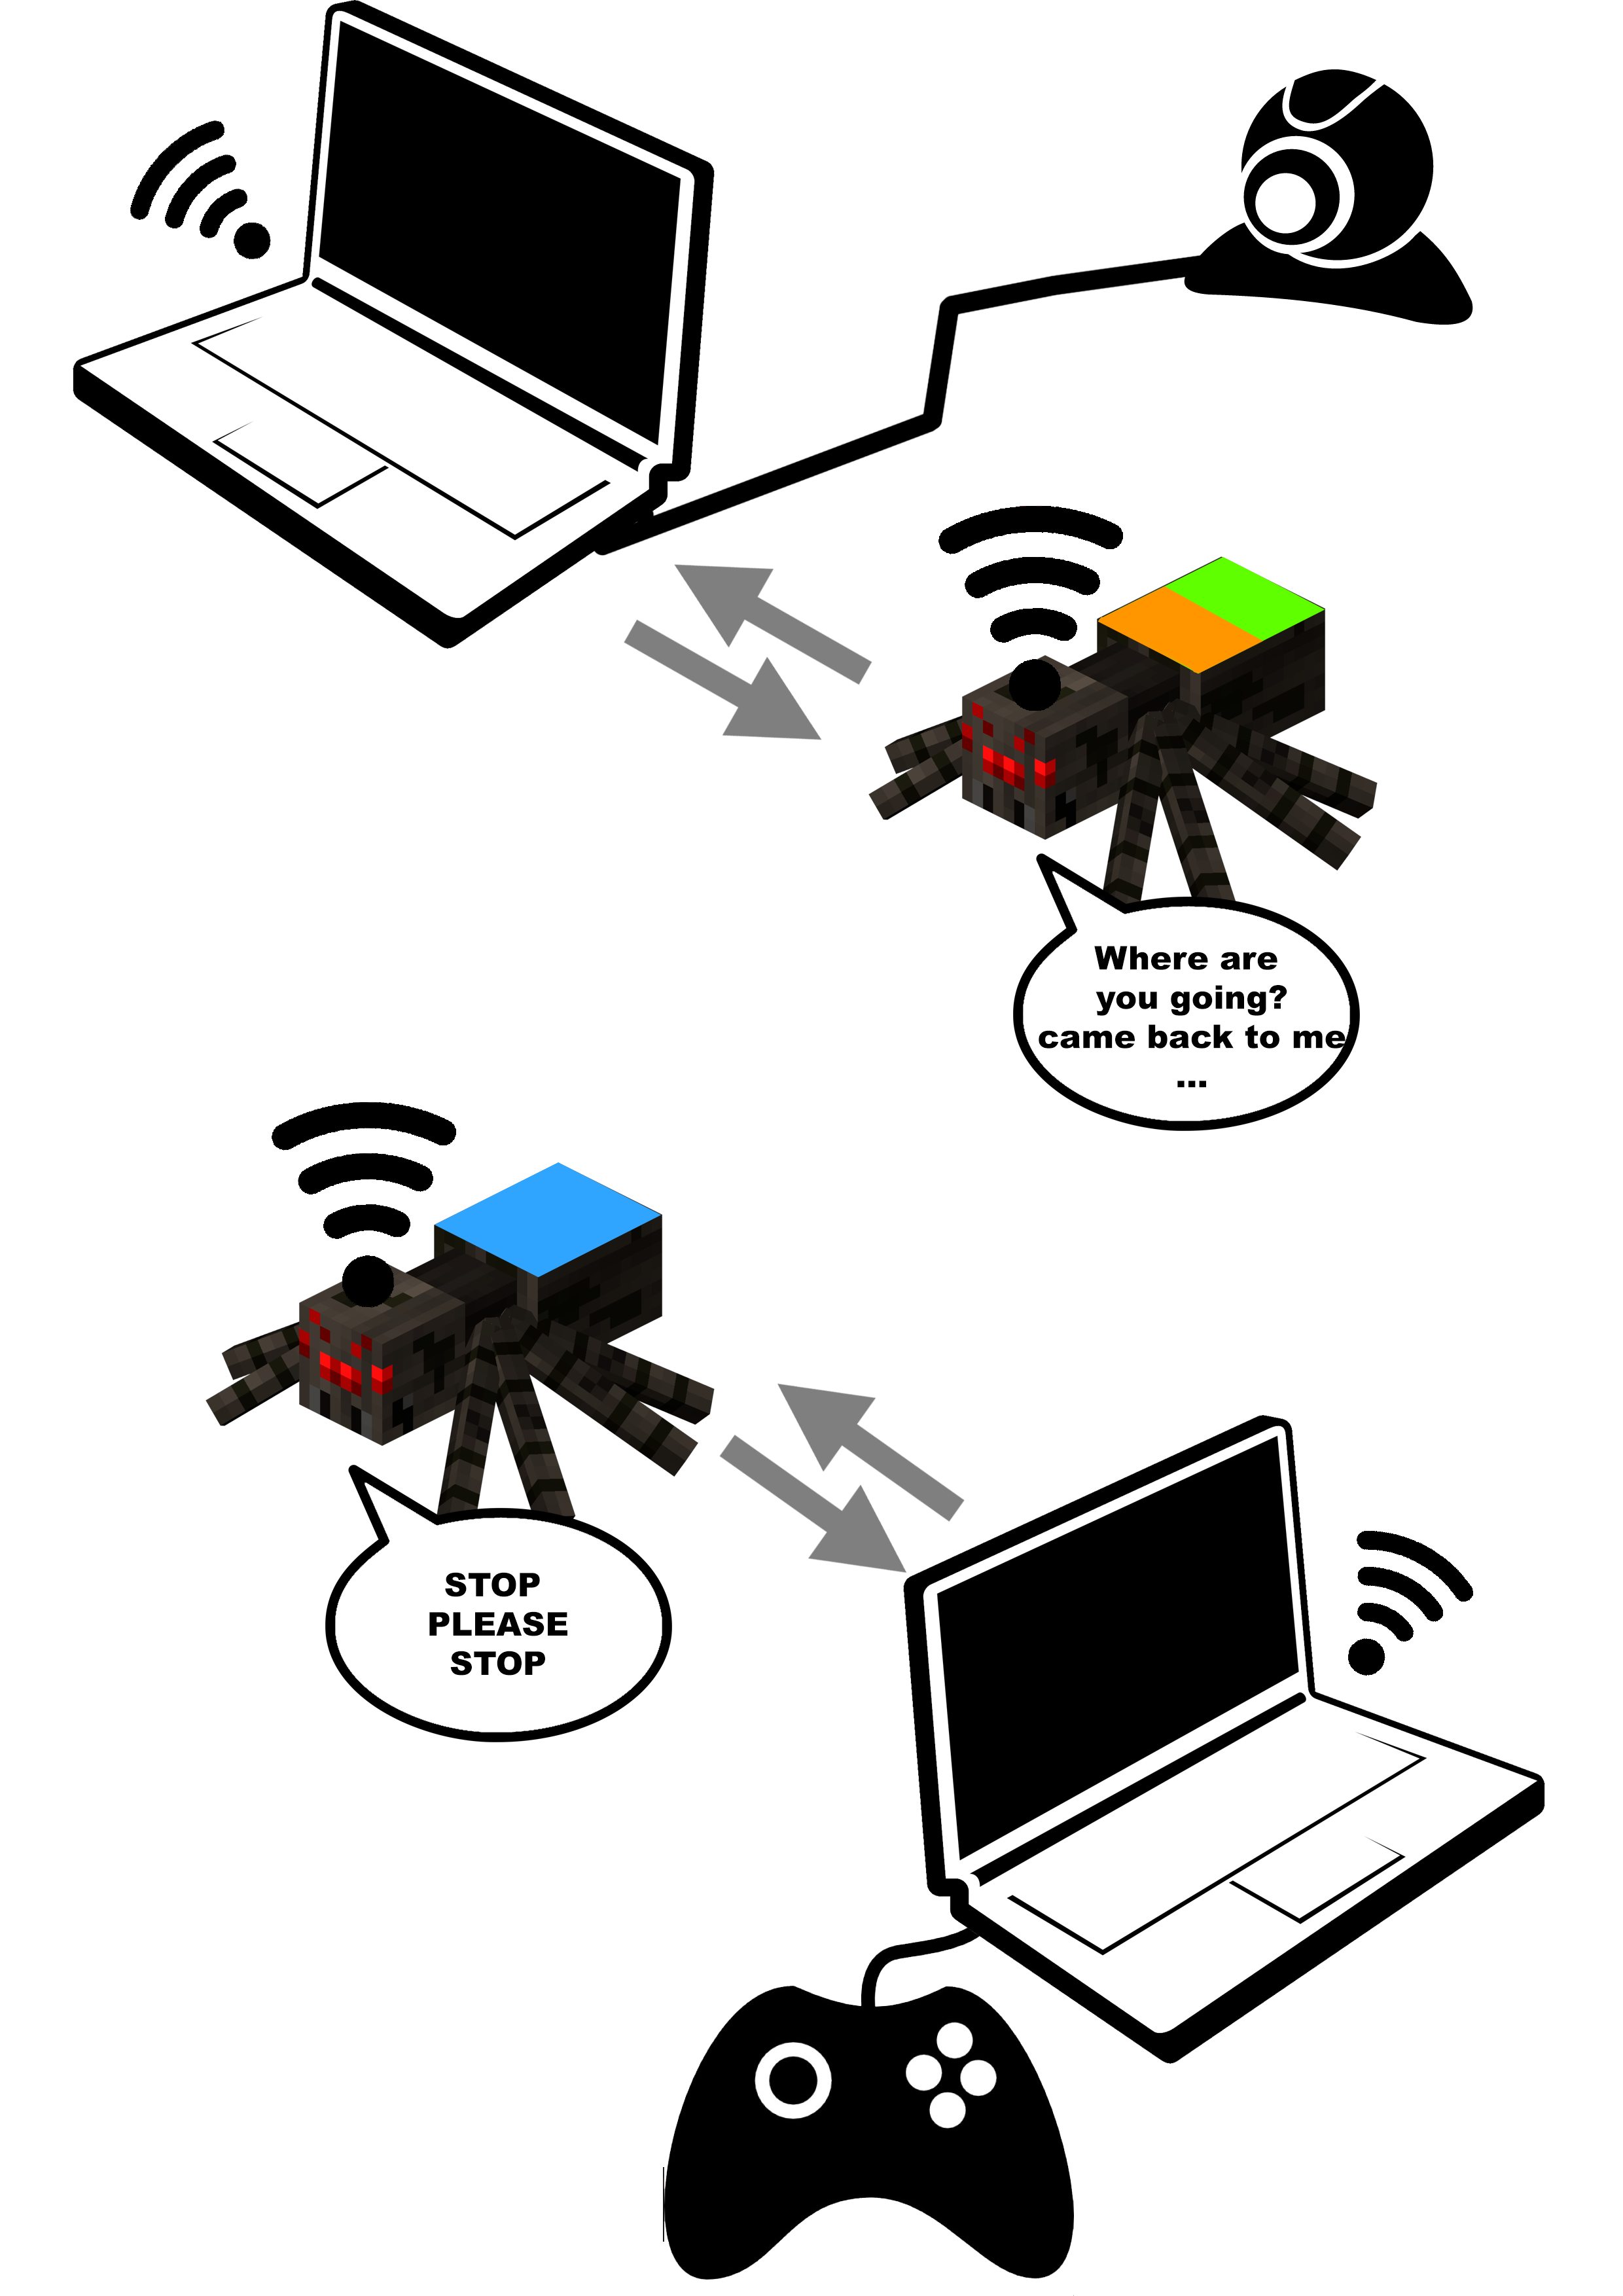
\includegraphics[keepaspectratio, width=200pt]{Images/Infographic.png}
\end{center}

Tutti e tre i ragni possono ricevere messaggi wireless che impostano le velocit\'a dei motori. Ricevuto il messaggio, la board regola le velocit\'a tramite il driver. Il requisito di localizzazione \'e soddisfatto da un modulo di visione artificiale: una webcam posta in alto riconosce i ragni, ed il pc alla quale \'e collegata invia messaggi direttamente ai ragni tramite WiFi. Inoltre, \'e possibile comandare i ragni tramite un cellulare Android od un pc, selezionando il ragno al quale si vogliono impartire i comandi. Ogni ragno \'e alimentato in maniera indipendente da 4 pile stilo poste in un portapile al di sotto del ragno stesso.

\subsection{Ragni meccanici}

I ragni meccanici che abbiamo comprato, mostrati in figura, utilizzano un solo motore per muovere sia le zampe a sinistra che quelle a destra. 
\begin{center}
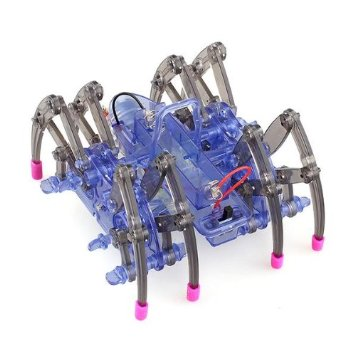
\includegraphics[keepaspectratio, width=300pt]{Images/single_spider2.png}
\end{center}
Bench\'e questa semplice soluzione sia sufficiente a far muovere il ragno avanti e indietro a velocit\'a prefisse, essa non andava incontro al nostro requisito di potersi muovere in qualsiasi direzione dello spazio. Per questo motivo, abbiamo rimosso le zampe a destra di tre ragni, e quelle di sinistra agli altri tre. Unendo i ragni cos\'i divisi, abbiamo ottenuto tre ragni totali, con il pregio di avere motori separati per zampa.
\begin{center}
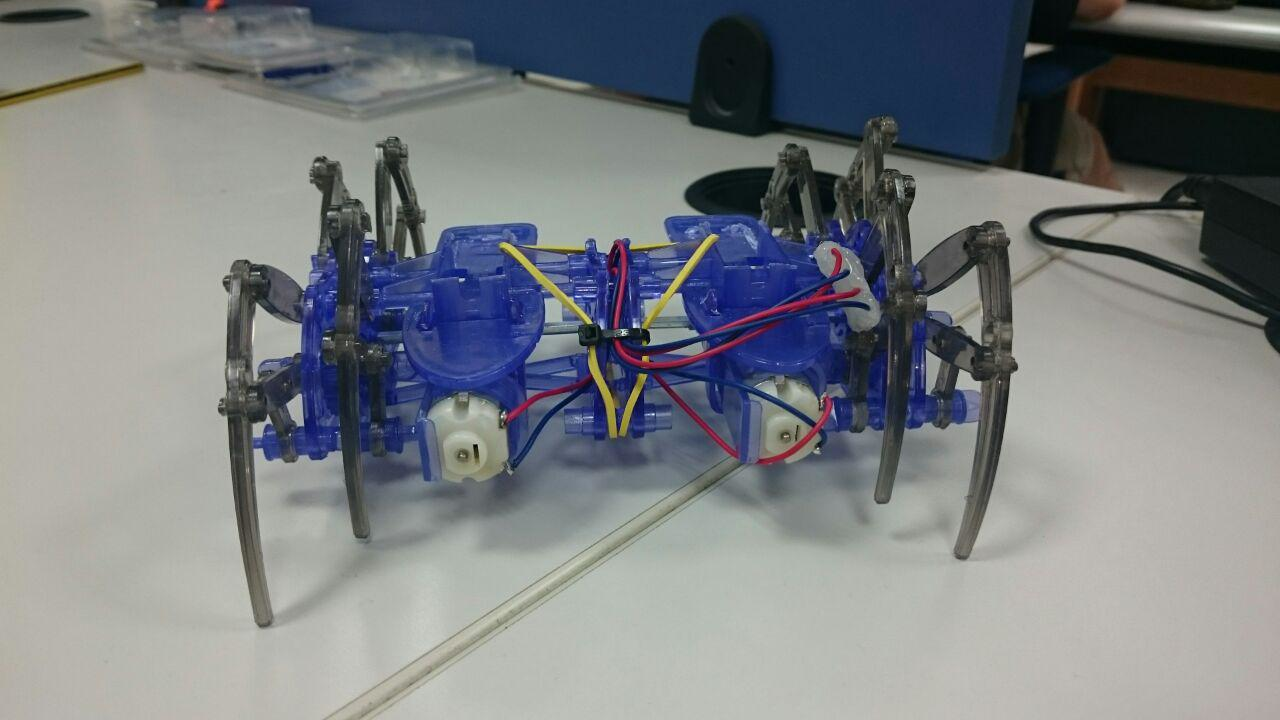
\includegraphics[keepaspectratio, width=300pt]{Images/double_spider.png}
\end{center}
\subsection{STM32F401RE Nucleo}
La board Nucleo STM32 fornisce un'infrastruttura affidabile e flessibile per gli utenti che vogliono sperimentare nuove idee e prototipi che funzionino con tutte la linea di microcontrollori STM32. Grazie al supporto per la connettivit\'a Arduino e ST Morpho, \'e possibile espandere le funzionalit\'a del microcontrollore scegliendo da una vasta gamma di shield. Inoltre, la STM32 nucleo non richiede due ingressi separati per alimentazione e debugging.
\begin{center}
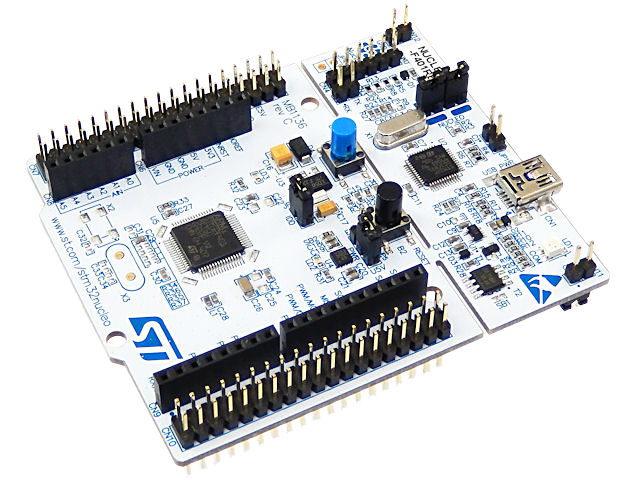
\includegraphics[keepaspectratio, width=200pt]{Images/STM32.png}
\end{center}
\subsection{Driver motore}
Il driver del motore utilizzato \'e il modello L9110s mostrato in figura. 
\begin{center}
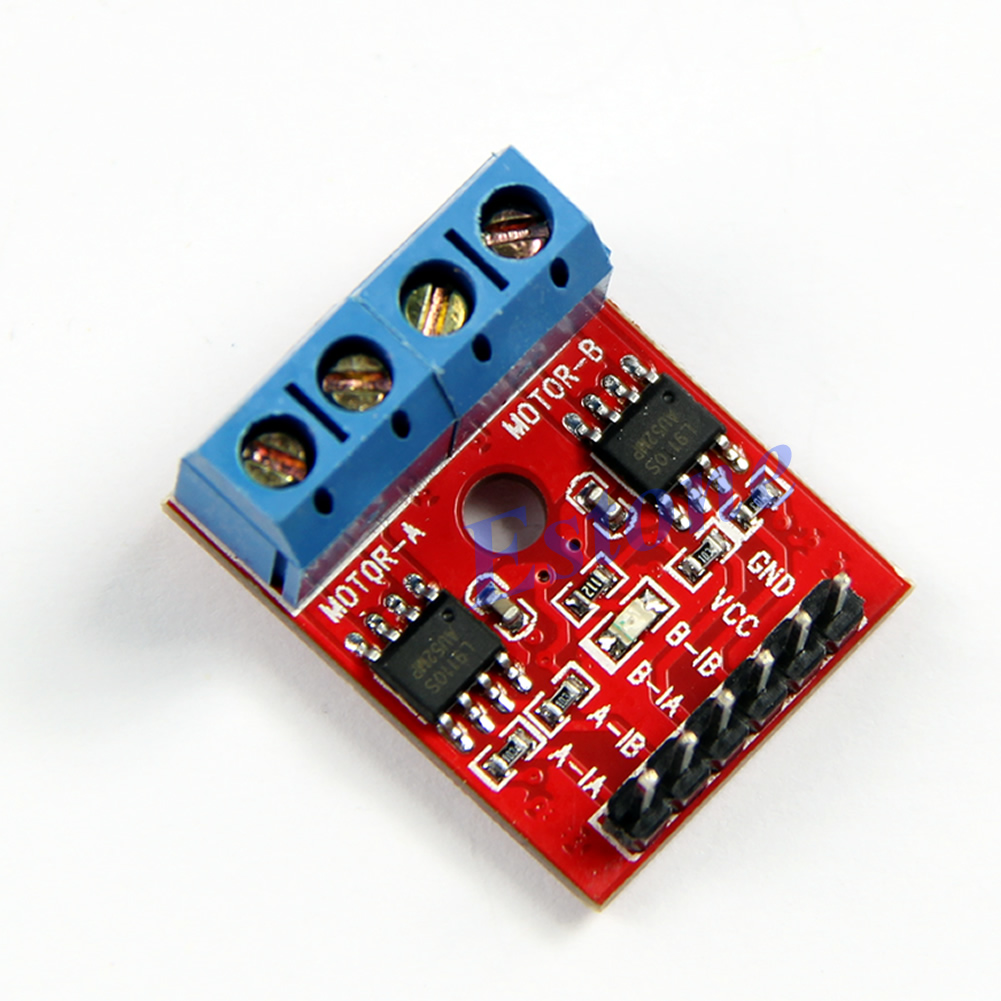
\includegraphics[keepaspectratio, width=200pt]{Images/motor_driver.png}
\end{center}
Dei suoi 10 pin totali, 4 sono di input e 4 di output, 1 di alimentazione e 1 di massa. Quelli in entrata vanno collegati agli output digitali della board, mentre di quelli in uscita 2 sono per il motore destro e 2 per quello sinistro, di cui 1 va all'alimentazione del motore ed uno alla massa. La regolazione della velocit\'a del motore \'e molto semplice e si basa sui PWM che sono collegati agli output digitali della board: se la frequenza del PWM  che arriva all'ingresso 1 \'e maggiore di quella che arriva all'ingresso 2, allora il ragno va in avanti, altrimenti va all'indietro. Maggiore \'e la differenza di velocit\'a, pi\'u il ragno va velocemente. Di seguito \'e riportato un diagramma riepilogativo.

\begin{center}
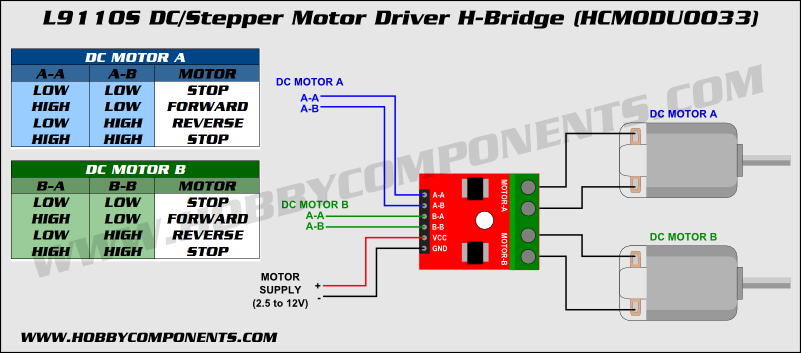
\includegraphics[keepaspectratio, width=400pt]{Images/motor_driver_diagram.png}
\end{center}

\subsection{Modulo wireless}
Il movimento dei robot \`e controllato da remoto tramite connessione wireless. La comunicazione wireless \`e garantita grazie ai moduli ESP8266 che, connessi alla board nucleo stm32f4, sono in grado di:
\begin{enumerate}
	\item connettersi ad una rete locale, acquisendo un indirizzo IP
	\item creare una connessione wireless locale
\end{enumerate}
In entrambi i casi, connettendosi alla rete del modulo \`e possibile scambiare messaggi tramite richieste http. Un semplice protocollo \`e stato realizzato per comandare i robot. L'idea \`e quella di codificare delle istruzioni di movimento in delle stringhe composte da 8 byte con il seguente significato:
\begin{itemize}
	\item il primo byte indica la tipologia di comando (attualmente \`e 'M' che sta per 'MOVE')
	\item il secondo byte \`e l'ID del robot; \`e stato pensato per robot connessi alla stessa rete
	\item 2 triple di 3 byte che codificano l'informazione di movimento relativamente per il motore destro e sinistro; una tripla pu\`o assumere un valore intero compreso tra 0 e 255: tra 0 e 127 si regola la velocit\`a di un motore in un senso; tra 128 e 255 si regola la velocit\`a del motore nell'altro senso
\end{itemize}
Il funzionamento del robot \`e descritto dal diagramma in figura \ref{fig:img}.
\begin{figure}
	\centering
		\hspace*{-4.9cm}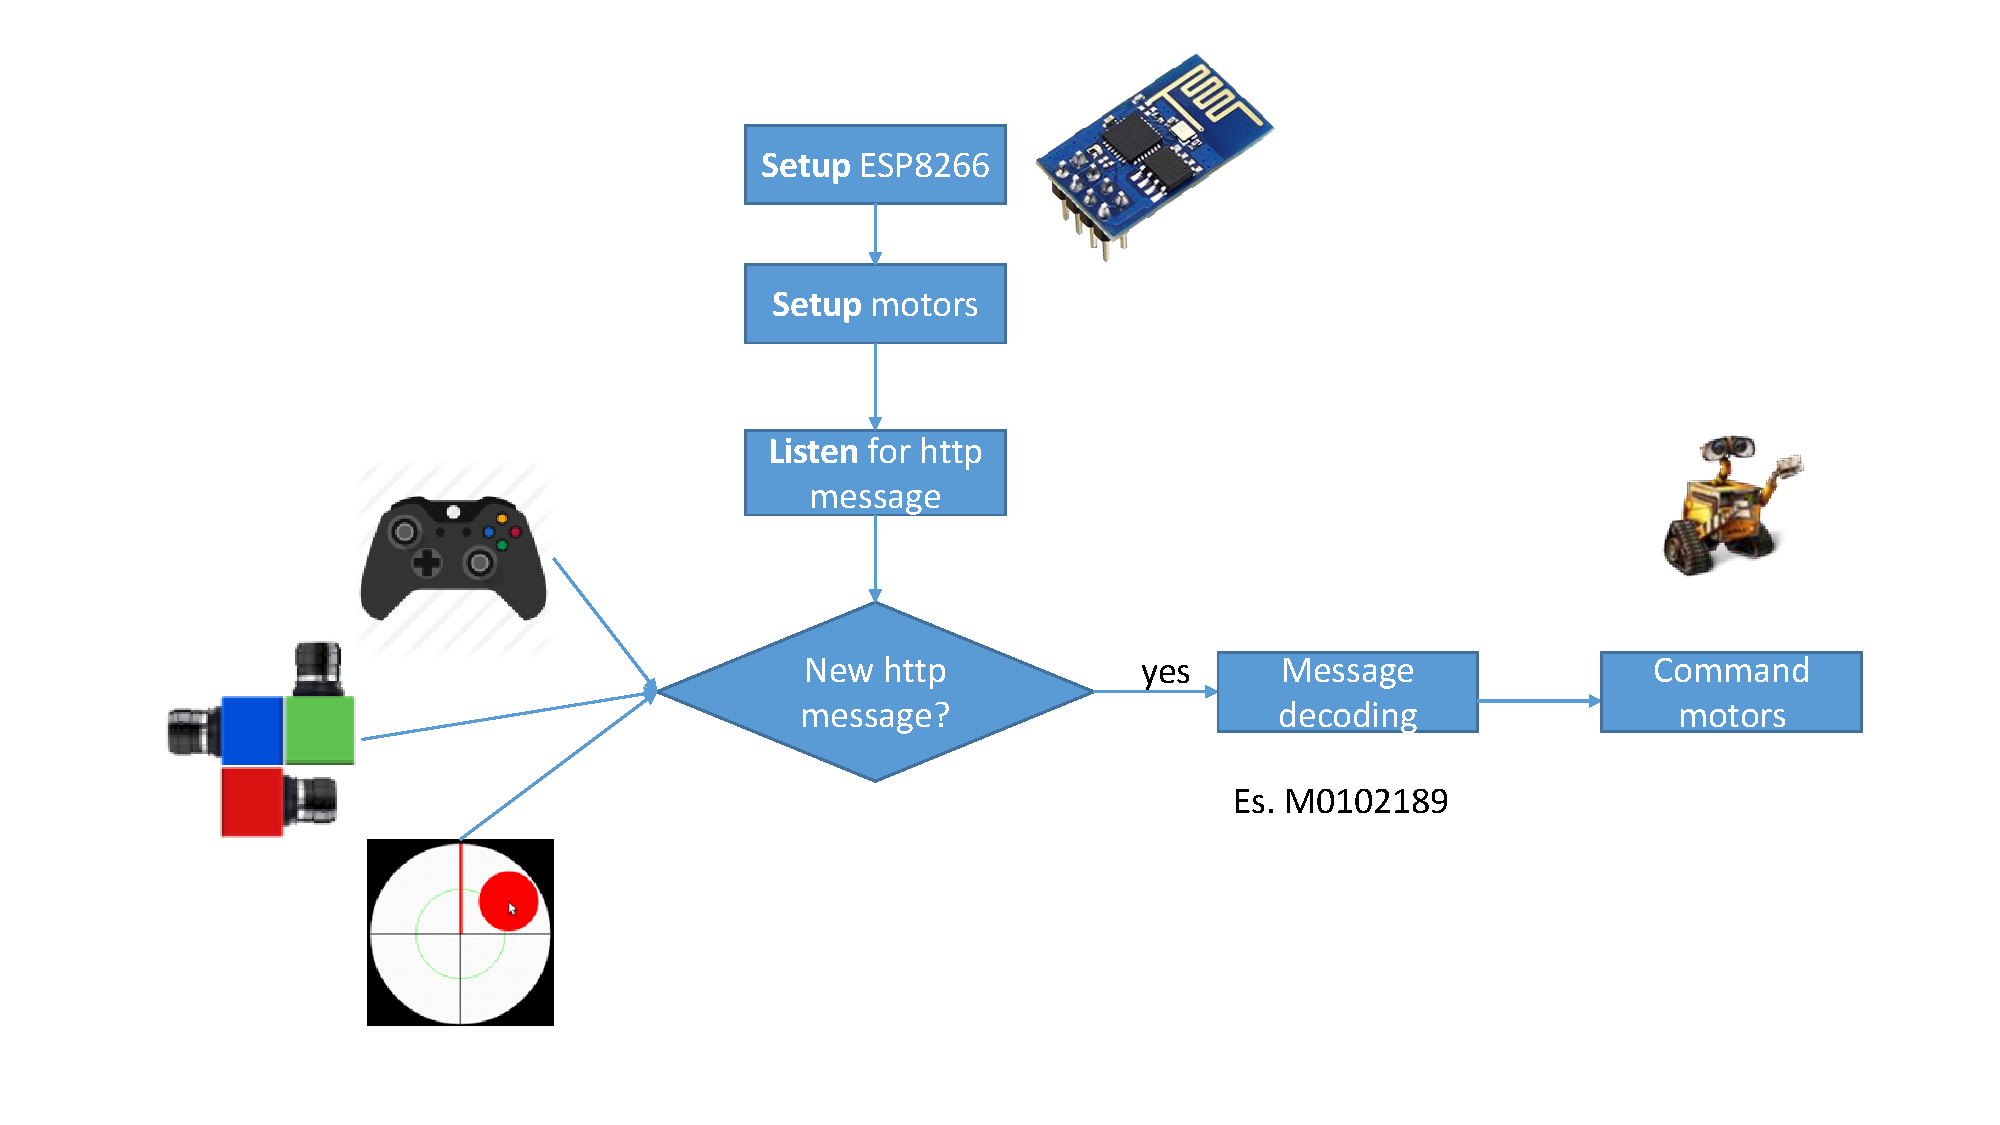
\includegraphics[width=1.7\textwidth]{Images/img.pdf}
		\caption{Il diagramma mostra lo schema di funzionamento della board che controlla il robot.}
	\label{fig:img}
\end{figure}

\section{Dettagli implementativi}

\subsection{Controller}

Per la comunicazione con i robot sono state utilizzate delle richieste http, con il formato descritto della sezione \ref{communication}. I due robot sono comandati rispettivamente da:	
\begin{itemize}
\item Soft-Joystick realizzato su Android (app Android) per il robot inseguito.
\item RoboWarsApp, una web app realizzata con nodeJS che consente di comandare il robot inseguito tramite tastiera o joystick xbox360.
\item Richieste http tramite python per il robot inseguitore.
\end{itemize}

\subsubsection{Android Controller}
L'app android utilizza una componente grafica che realizza un Joystick (\url{https://github.com/zerokol/JoystickView}) e, a seconda della direzione del Joystick, invia richieste http al modulo ESP8266 con il formato descritto in \ref{communication}. L'immagine in figura \ref{fig:joy} mostra la semplice interfaccia grafica dell'app Android per il controllo del robot.

\begin{figure}
	\centering
		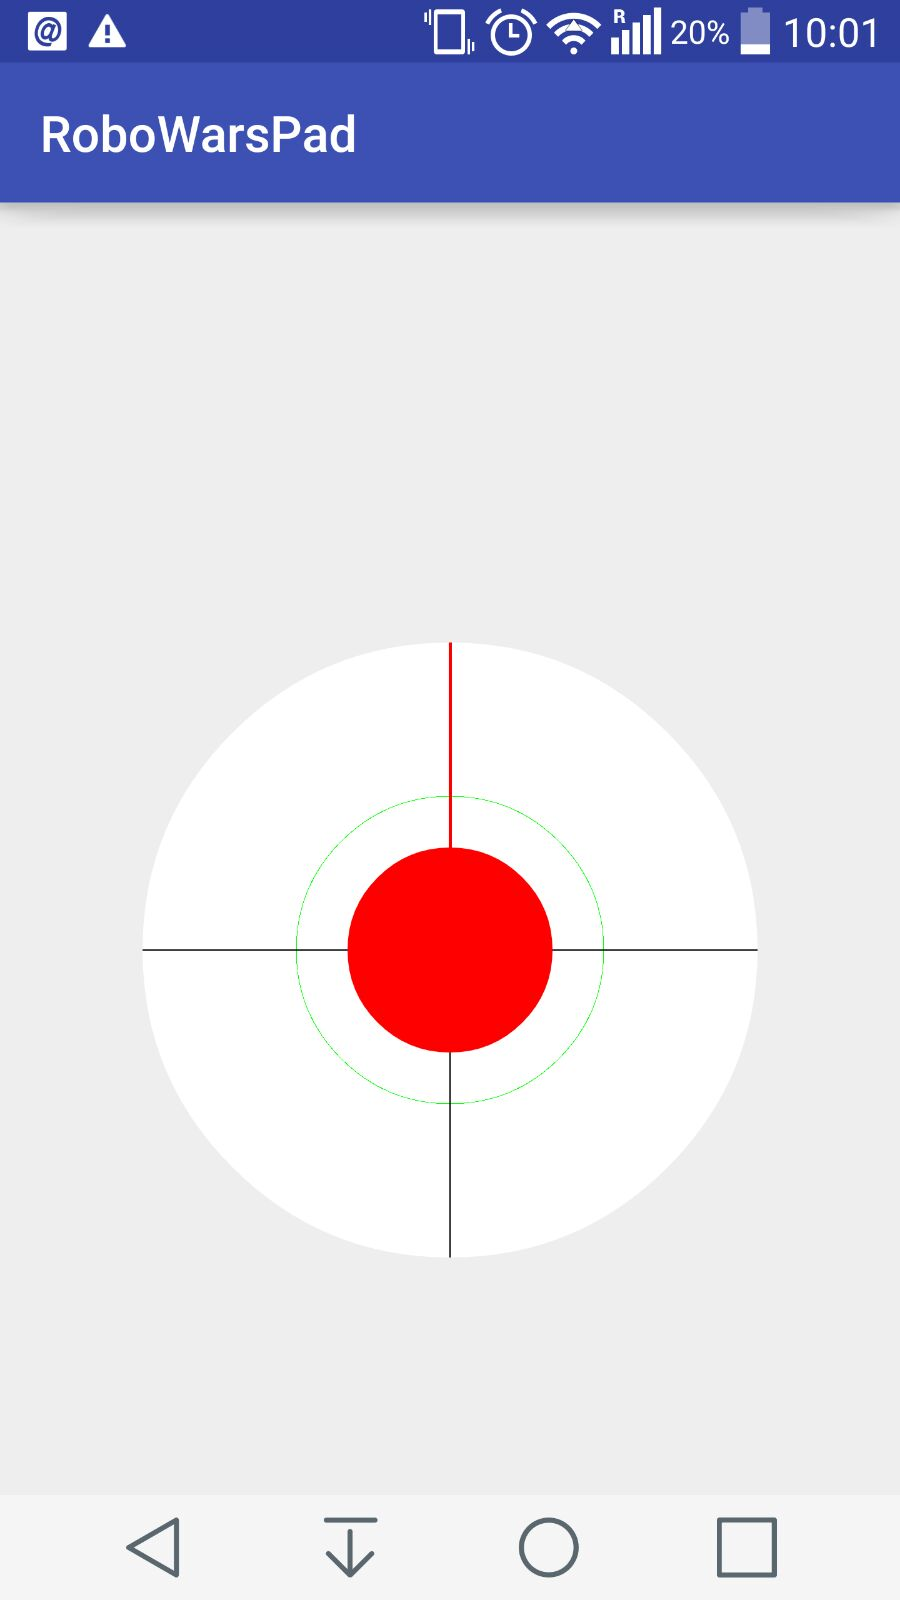
\includegraphics[width=0.4\textwidth]{Images/joy.jpg}
	\label{fig:joy}
	\caption{L'immagine mostra l'intercaccia grafica del controller Android realizzato per comandare il robot.}
\end{figure}

\subsubsection{RoboWarsApp}
La web app sviluppata consiste nella semplice interfaccia mostrata in figura.

\begin{center}
\end{center}

\subsection{Driver motore}

Il driver del motore contiene la funzione di inizializzazione, la funzione di controllo del motore date le velocit\'a, ed una funzione di utilit\'a che estrae le due velocit\'a a partire da una stringa.

\lstinputlisting[caption=Motor Driver, style=c]{../RoboWars/MotorController.h}

\subsection{Modulo wireless}

 Per l'utilizzo della board con il sistema ChibiOS \`e stata realizzata una apposita libreria che racchiude diverse funzionalit\`a. Il modulo ESP8266 pu\`o essere configurato tramite comandi seriali (vedi \ref{fig:commands}). Per ogni comando, il modulo genera una risposta che pu\`o essere un ACK o un messaggio di errore.
La libreria consente la configurazione del modulo come Access Point o come client (fornendo le credenziali di accesso ad una rete Wi-Fi) tramite due semplici funzioni. Chiamando qualsiasi di queste due funzioni, viene creato un Thread asincrono che rimane in ascolto di eventi sulla seriale a cui \`e collegato il modulo ESP8266. Nel caso specifico i moduli sono stati utilizzati come Access Point.
I comandi fondamentali inviati in fase di setup sono:
\begin{itemize}
	\item comando di reset: "AT+RST"
	\item comando di setup della modalit\`a di funzionamento: "AT+CWMODE=2" (per modalit\`a access point)
	\item comando di start del server:  "AT+CIPSERVER=1,80";
\end{itemize}
Maggiori dettagli sui comandi disponibili sono mostrati nella tabella \ref{fig:commands}.
\par Quando viene inviata una richiesta http al modulo, viene generato un evento sulla seriale e viene costruita la stringa con il messaggio ricevuto. Tale messaggio \`e composto da una intestazione e da una cosa. Un parser del messaggio \`e stato realizzato per estrarre la stringa di interesse (es. M0123200); decodificato il messaggio viene invocato il metodo 'control\_motor' della libreria 'MotorController.h' che prende in carico la richiesta e comanda i motori.
\par Oltre alla seriale utilizzata per comunicare con l'ESP8266, la libreria utilizza anche la seriale USB per stampare a video i messaggi ricevuti dal modulo in tempo reale. Tale meccanismo \`e utile in fase di debug per conoscere lo stato del modulo ed intercettare eventuali errori. 

\begin{figure}
	\centering
		\hspace*{-2cm}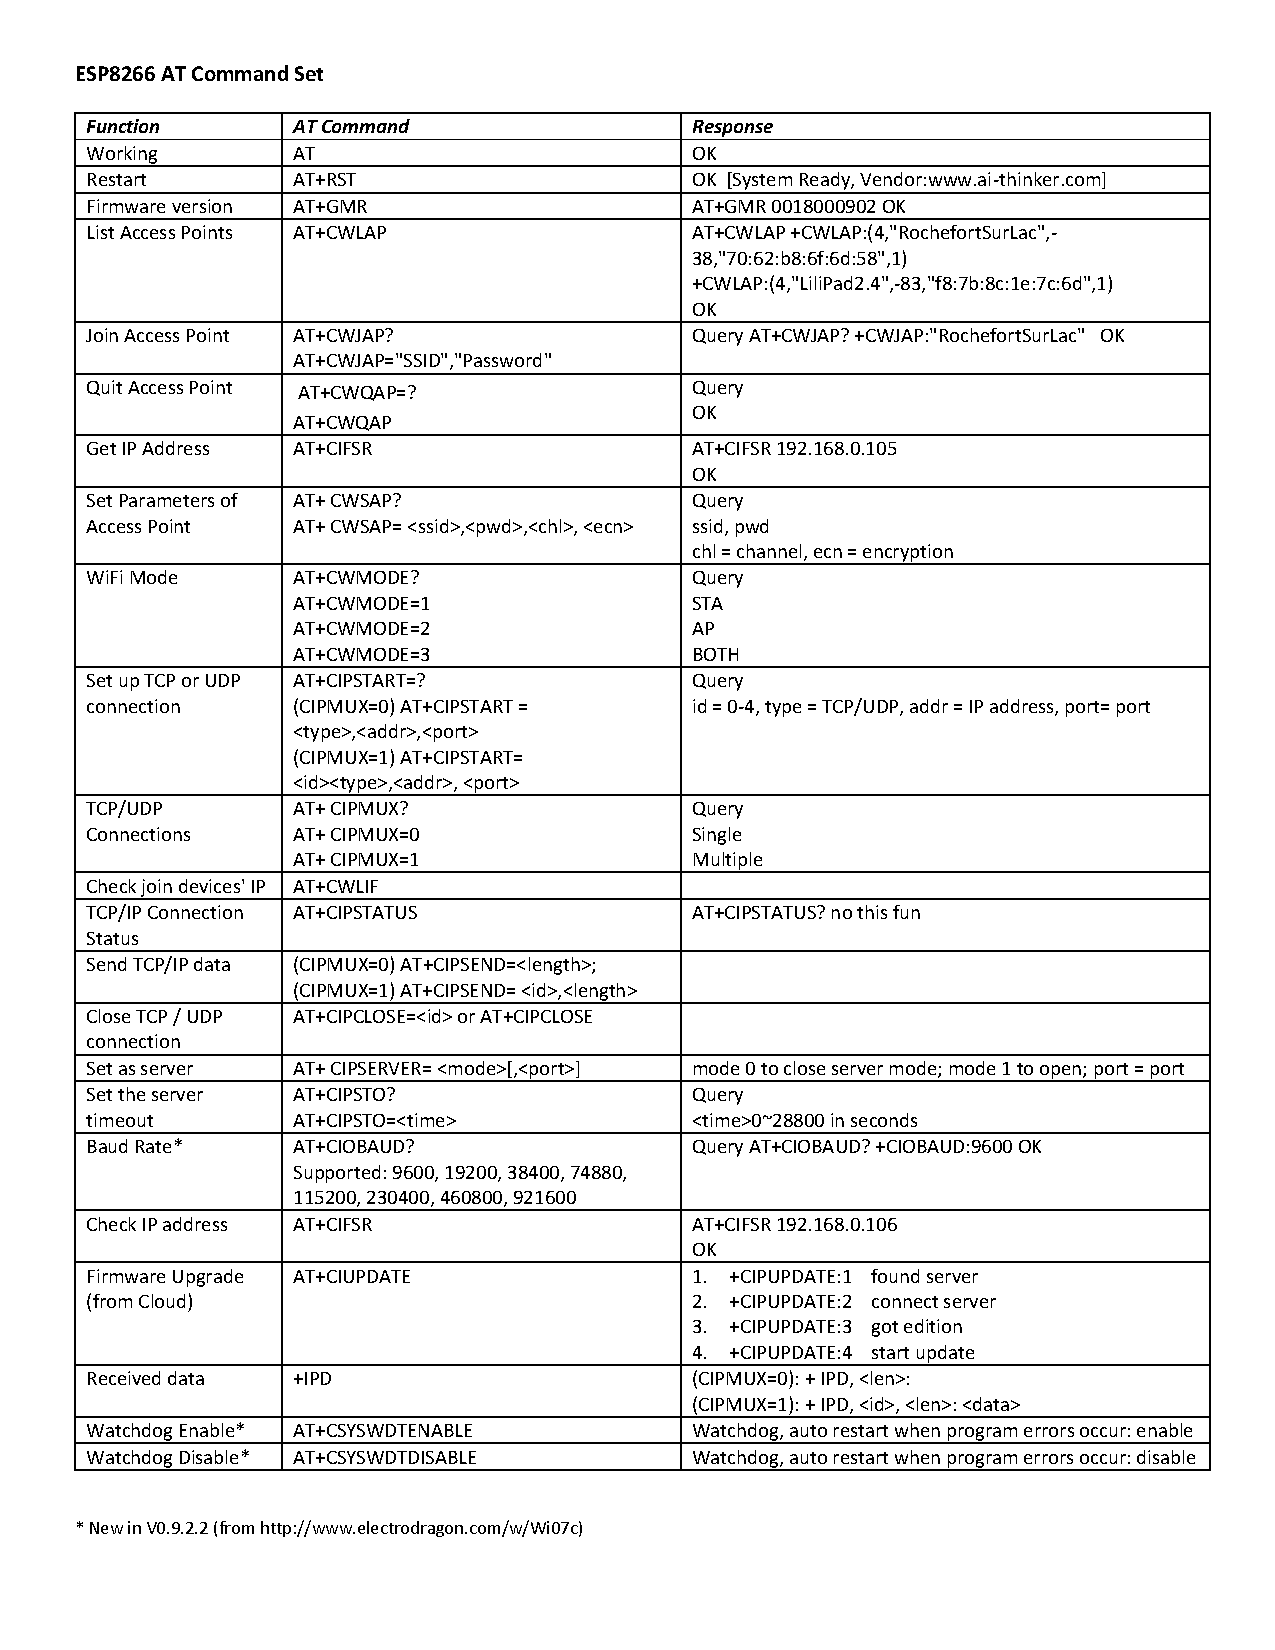
\includegraphics[width=1.30\textwidth]{Images/CommandsSet.pdf}
	\label{fig:commands}
	\caption{La tabella contiene i comandi riconosciuti dal modulo ESP8266 con relativa risposta.}
\end{figure}

\lstinputlisting[caption=Module, style=c]{../RoboWars/ESP8266.h}

\subsection{Visione Artificiale}

\lstinputlisting[caption=Vision, style=python]{../Vision/Vision.py}

\section{Conclusioni}

\subsection{Sviluppi futuri}
Il progetto sviluppato ha soddisfatto appieno i requisiti funzionali che ci siamo preposti. Tuttavia, alcuni aspetti potranno essere sicuramente migliorati in futuro:
\begin{itemize}
\item I cartoncini colorati potranno essere sostituiti da markers per la realt\'a aumentata. Ci\'o migliorer\'a il riconoscimento dei ragni ed eliminer\'a la necessit\'a del doppio colore per stabilire l'orientamento del ragno inseguitore. 
\item L'algoritmo di inseguimento potr\'a essere migliorato pianificando traiettorie di curvatura e aggiungendo a bordo del ragno un sensore di prossimit\'a.
\item Si potrebbe eliminare la necessit\'a di un sistema di orientamento globale montando una webcam direttamente sui ragni.
\end{itemize}

\end{document}